% Created 2025-09-24 Wed 21:19
% Intended LaTeX compiler: pdflatex
\documentclass[11pt]{article}
\usepackage[utf8]{inputenc}
\usepackage[T1]{fontenc}
\usepackage{graphicx}
\usepackage{longtable}
\usepackage{wrapfig}
\usepackage{rotating}
\usepackage[normalem]{ulem}
\usepackage{amsmath}
\usepackage{amssymb}
\usepackage{capt-of}
\usepackage{hyperref}
\author{Russo Antonio}
\date{2025-09-22}
\title{Distributed Virtual File System (DVFS)}
\hypersetup{
 pdfauthor={Russo Antonio},
 pdftitle={Distributed Virtual File System (DVFS)},
 pdfkeywords={},
 pdfsubject={},
 pdfcreator={Emacs 30.2 (Org mode 9.7.11)}, 
 pdflang={English}}
\begin{document}

\maketitle
\tableofcontents

\section{Introduzione}
\label{sec:org0fc3aaa}
Il \textbf{Distributed Virtual File System (DVFS)} è un progetto che implementa un file system distribuito secondo un modello \textbf{client-server}.  
L’idea di base è permettere a più client di accedere a un file system remoto come se fosse locale, con un’interfaccia semplice e coerente.  
Il sistema è sviluppato in \textbf{Java} ed utilizza \textbf{RMI (Remote Method Invocation)} come meccanismo di comunicazione, garantendo trasparenza delle invocazioni e modularità.  

Il DVFS offre funzionalità classiche di un file system (creazione, lettura, scrittura, navigazione) e introduce una politica di \textbf{write-through}, che assicura che ogni modifica in memoria venga immediatamente riflessa anche sul file system reale montato sul server.  
\section{Architettura}
\label{sec:org1315a3c}
L’architettura segue il modello \textbf{client-server centralizzato}:

\begin{itemize}
\item \textbf{FileSystem}: cuore del sistema, un file system virtuale in memoria strutturato come un albero. Ogni nodo può rappresentare directory, file o symlink. Le operazioni in memoria vengono sincronizzate su disco tramite write-through.
\item \textbf{RemoteFileSystem}: oggetto RMI che funge da “ponte” tra i client e il VFS locale. Implementa l’interfaccia remota e inoltra le richieste al FileSystem.
\item \textbf{FileSystemServer}: avvia e monta il VFS da una directory reale, pubblica lo stub RMI e resta in ascolto delle richieste.
\item \textbf{FileSystemClient}: applicazione a riga di comando che permette di interagire col file system remoto. Supporta comandi familiari (\textbf{mkdir}, \textbf{ls}, \textbf{read}, \textbf{write}) e funzionalità avanzate come \textbf{edit}, che scarica un file remoto in un editor locale e lo risincronizza al termine della modifica.
\end{itemize}

Questa separazione isola le responsabilità: i client gestiscono l’interazione con l’utente, mentre il server centralizza la logica del file system e garantisce consistenza tra più richieste concorrenti.  

\begin{figure}[htbp]
\centering
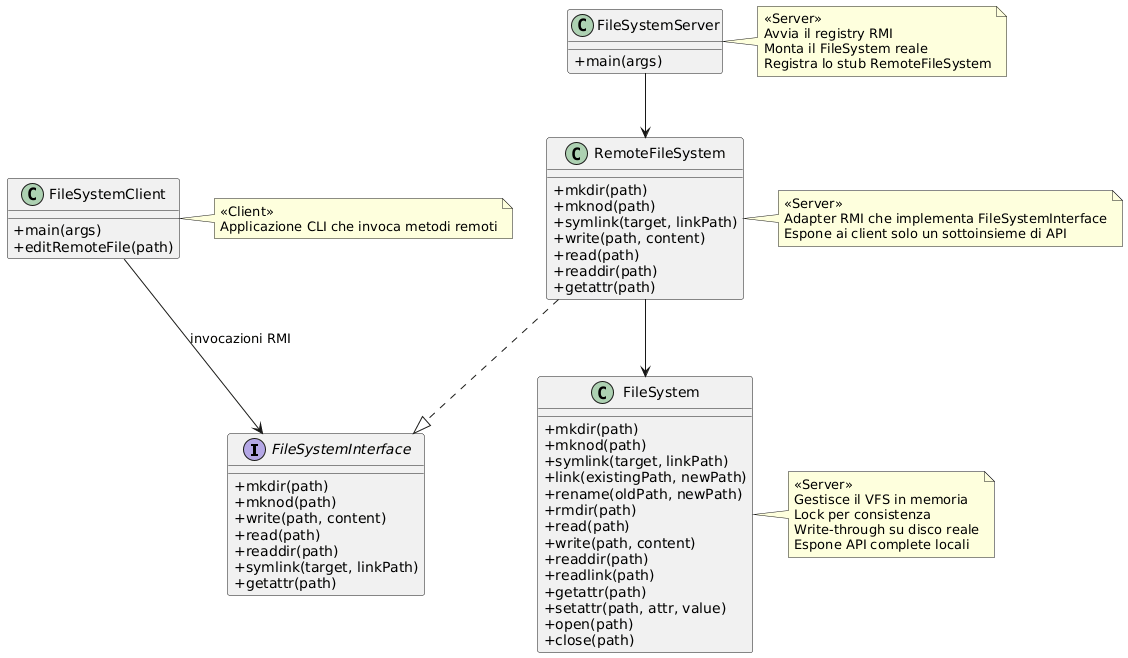
\includegraphics[width=.9\linewidth]{img/arch.png}
\caption{Architettura client-server DVFS}
\end{figure}
\section{Consistenza}
\label{sec:org1744541}
La consistenza è garantita dal \textbf{server}.  
Ogni operazione che modifica lo stato (scrittura, rinomina, rimozione) viene protetta da lock a livello di path (\textbf{ReentrantReadWriteLock}).  

\begin{itemize}
\item Più client possono leggere contemporaneamente senza conflitti.
\item Le scritture sono serializzate, impedendo \textbf{race condition}.
\item Ogni modifica avviene in due fasi: aggiornamento in memoria e write-through su disco.
\end{itemize}

I client non gestiscono lock: tutta la concorrenza viene risolta dal server, che possiede l’unica copia “autorevole” dello stato.  
\section{Montaggio da directory reale}
\label{sec:org587691f}
Il sistema può partire da zero o essere montato da una directory esistente.  
In questo caso, il contenuto viene caricato ricorsivamente:  

\begin{itemize}
\item Directory → DirectoryNode.
\item File → FileNode (contenuto letto in memoria).
\item Symlink → SymlinkNode (target salvato).
\end{itemize}

La root del VFS viene rinominata “/”, e ogni operazione successiva (scrittura, rinomina, rimozione) viene riflessa anche sulla directory reale tramite write-through.  
\section{Funzionalità}
\label{sec:org67798ae}
Il DVFS mette a disposizione un set completo di operazioni:  

\begin{itemize}
\item \textbf{Creazione}: mkdir, mknod, symlink, link.
\item \textbf{Navigazione}: lookup, readdir, readlink.
\item \textbf{Manipolazione}: read, write, rename, rmdir.
\item \textbf{Gestione attributi}: getattr, setattr.
\item \textbf{Gestione apertura/chiusura}: open, close.
\end{itemize}

Inoltre, lato client è disponibile il comando \textbf{edit}, che consente di modificare un file remoto con un editor locale in maniera trasparente.  
\section{Protocolli}
\label{sec:org151bc62}
La comunicazione tra client e server avviene tramite \textbf{Java RMI}.  
Le invocazioni remote sono trasparenti: il client invoca metodi sull’interfaccia \textbf{FileSystemInterface}, che vengono eseguiti dal server sul VFS locale.  
\subsection{Flusso tipico di un’operazione}
\label{sec:orgd02ae1e}
\begin{enumerate}
\item Il client invia una richiesta remota (es. \texttt{write("/foo", data)}).
\item Lo stub RMI inoltra la chiamata a RemoteFileSystem sul server.
\item RemoteFileSystem chiama il metodo corrispondente di FileSystem.
\item FileSystem acquisisce il lock, aggiorna lo stato in memoria e riflette la modifica su disco.
\item Il risultato viene restituito al client.
\end{enumerate}

\begin{figure}[htbp]
\centering
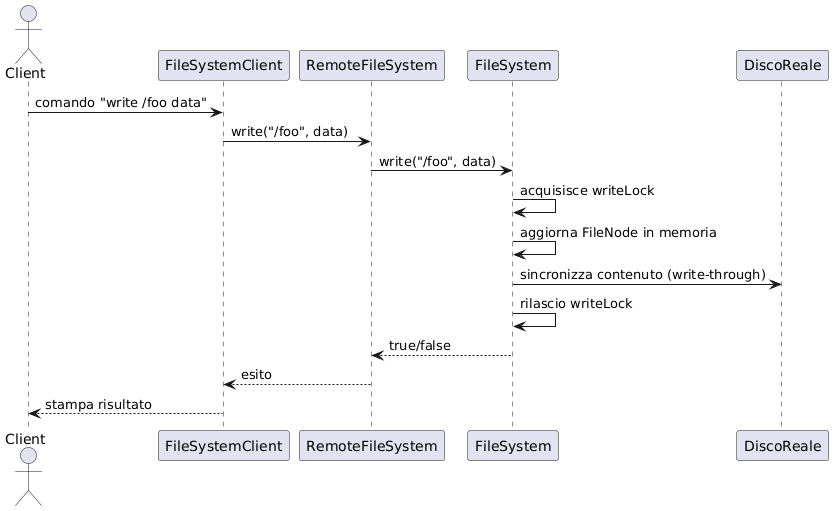
\includegraphics[width=.9\linewidth]{img/uml_op.png}
\caption{Flusso di una richiesta write}
\end{figure}
\section{Sicurezza ed error handling}
\label{sec:orga2a36d9}
\begin{itemize}
\item Durante la risoluzione dei path, il server impedisce accessi fuori dalla root montata (protezione da path traversal).
\item In caso di errori I/O durante il write-through, l’operazione resta valida in memoria, evitando perdita di dati.
\item Gli errori lato server vengono propagati al client come eccezioni RMI.
\end{itemize}
\subsection{Diagramma UML delle classi}
\label{sec:org5970416}
\section{Protocolli usati}
\label{sec:org733059d}
Il sistema utilizza Java RMI come protocollo client-server:
\begin{itemize}
\item I client invocano metodi remoti sull’oggetto RemoteFileSystem.
\item Il server centralizza la gestione dei lock e della consistenza.
\item I client non comunicano direttamente tra loro (no peer-to-peer).
\end{itemize}
\end{document}
